%&pdflatex

\documentclass{article}
\usepackage{bera}% optional: just to have a nice mono-spaced font
\usepackage{listings}
\usepackage{xcolor}
\usepackage{pdfpages}

\begin{document}
  \title{StoreIt Protocol v0.2}
  \author{Adrien Morel \texttt{adrien.morel@me.com}}
  \date{\today}
  \maketitle

\section{Introduction}

Hello, this is the documentation for the StoreIt protocol. It is used when two clients talk and when the clients and the server talk.\\
\textbf{Everything which is not some binary data (chunks) should be encoded in ASCII.} Everything in the protocol is ether a \textit{command} or a \textit{numeric response}. A command will always have the following structure:\\
\begin{center}
\textbf{NAME} SIZE \textit{arg1 [arg2 arg3...]} [payload]
\end{center}

\begin{itemize}
  \item NAME is the command name. "JOIN" for example. Every command name is ALWAYS 4 characters long.
  \item SIZE is the size in bytes following the ' ' (space) after SIZE. For example \textit{TAKE 9 money 900}.
  \item \textit{arg} are command ASCII arguments.
  \item payload is a list of bytes for some payload. Example :\\
\begin{lstlisting}
 STORE 18 hi.txt hello world
\end{lstlisting}
Here, "hello world" is the payload and "hi.txt" is an argument.
\end{itemize}
When I write [client] -> [server] it means "this command is sent by a client to our backend servers". [client] -> [client] means "it is sent from client to client" (p2p).\\
\section{The JSON data structures}
\subsection{File Object}

\colorlet{punct}{red!60!black}
\definecolor{background}{HTML}{EEEEEE}
\definecolor{delim}{RGB}{20,105,176}
\colorlet{numb}{magenta!60!black}

\lstdefinelanguage{json}{
    basicstyle=\normalfont\ttfamily,
    numbers=left,
    numberstyle=\scriptsize,
    stepnumber=1,
    numbersep=8pt,
    showstringspaces=false,
    breaklines=true,
    frame=lines,
    backgroundcolor=\color{background},
    literate=
     *{0}{{{\color{numb}0}}}{1}
      {1}{{{\color{numb}1}}}{1}
      {2}{{{\color{numb}2}}}{1}
      {3}{{{\color{numb}3}}}{1}
      {4}{{{\color{numb}4}}}{1}
      {5}{{{\color{numb}5}}}{1}
      {6}{{{\color{numb}6}}}{1}
      {7}{{{\color{numb}7}}}{1}
      {8}{{{\color{numb}8}}}{1}
      {9}{{{\color{numb}9}}}{1}
      {:}{{{\color{punct}{:}}}}{1}
      {,}{{{\color{punct}{,}}}}{1}
      {\{}{{{\color{delim}{\{}}}}{1}
      {\}}{{{\color{delim}{\}}}}}{1}
      {[}{{{\color{delim}{[}}}}{1}
      {]}{{{\color{delim}{]}}}}{1},
}

\begin{lstlisting}[language=json,firstnumber=1]
{
  "path": "storeit",
  "metadata": "unimplemented for now",
  "unique_hash": "sha256 hash of all the data in the file",
  "kind": 0,

  // for now, this list is not necessary.
  "chunks_hashes": [
    "some sha256"
  ],
  "files": {
    "file_name": anotherFileObject,
    "another_file_name": anotherFileObject
  }
}
\end{lstlisting}

\section{ASCII Commands}

\subsection{Session}

\paragraph{JOIN}

[client] -> [server]\\
This is the first request to make whenever a client wants to get online.\\
\begin{center}JOIN SIZE username port json\_file\end{center}
Json\_file is the json tree describe in the second section.

\paragraph{QUIT}

[client] -> [server]\\
A client should send this to our server to leave the network.\\

\begin{center}QUIT 0\end{center}

Note that '0' is the SIZE parameter. It is always zero since there is no argument.\\

\subsection{Raw Data Manipulation (chunks)}

\paragraph{CDEL (chunk delete)}

[server] -> [client]\\
The server asks the client to delete a chunk it is storing.

\begin{center}CDEL SIZE chunk\_hash\end{center}

\paragraph{CSND (chunk send)}

[server] -> [client]\\
 Tells a client to wait for a specific client to send it a chunk (only in the case of chunks that don't belongs to a user), or to send a chunk to another client. See the diagram at the end of the document to better understand.

\begin{center}CSND SIZE send chunk\_hash ip\_address:port\end{center}

\begin{itemize}
  \item send: \begin{itemize}
    \item 0: should wait for incoming chunk.
    \item 1: should send the chunk to the specified client.
    \end{itemize}
  \item chunk\_hash: the chunk's hash
  \item ip\_address:port: the ip address and port of the client that should be contacted.
\end{itemize}
    
\paragraph{CSTR (chunk store)}
[client] -> [client]\\
Send a chunk to a client.

\begin{center}CSTR SIZE payload\end{center}

Payload is the chunk bytes.

\subsection{File Management}

\paragraph{FDEL (file delete)}

[client] -> [server] or [server] -> [client] \\
Delete a file/directory.\\

\begin{center}FDEL SIZE file\_path\end{center}

\paragraph{FADD (file add)}

[client] -> [server] or [server] -> [client] \\

Add a file to the user tree. If it is sent from the server, the user should create the file and wait further instructions to fetch the file data. Otherwise if it is sent from the client, the server will attempt to add the file to the user virtual tree. It will then send further instructions to dispatch the data on the network. See the diagram for better understanding.\\

\begin{center}FADD SIZE json\_file\end{center}

\paragraph{FUPT (file update)}

[client] -> [server] or [server] -> [client] \\
Tell the server to update a file, or receive the order to update a file. Like FADD, it will be followed by further instructions to get the raw data.

\begin{center}FUPT SIZE json\_file\end{center}

\section{Numeric responses}

textbf{This is not yet implemented on the server so don't implement it for now.}
Just send '0 0' if everything went well (it's the command '0' with size 0. Send '1' SIZE 'error message' if something wrong occured and you could not complete the command.

\section{Examples Diagrams}

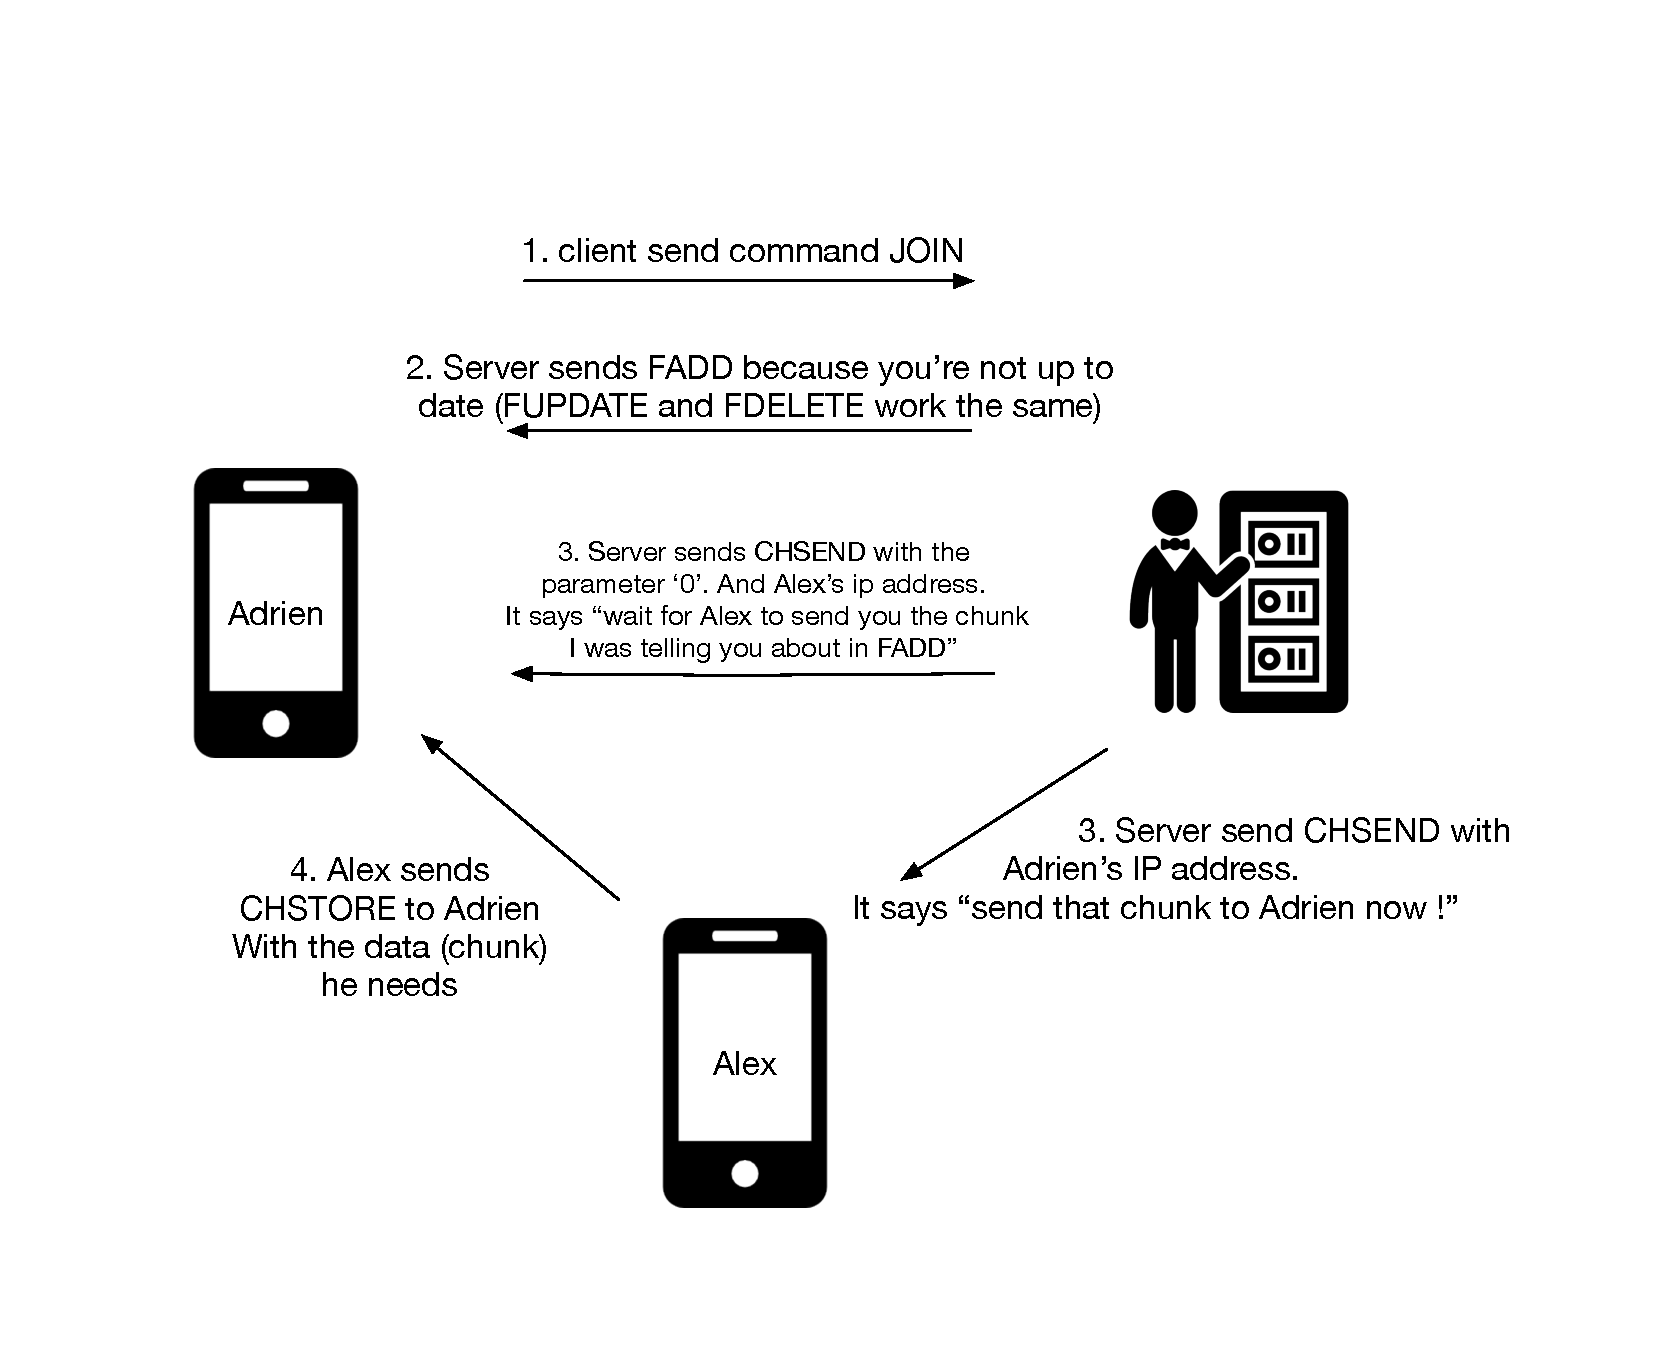
\includepdf{diagram.pdf}

\end{document}
